\documentclass[UTF8]{beamer}
\usepackage{graphicx, color}
\usepackage{algorithm2e}
\usepackage{zhspacing}
\usepackage{amsmath}

\usepackage{underscore}
\usetheme{JuanLesPins}
\usepackage{fontspec}
\setsansfont{Microsoft YaHei}

\usepackage{enumerate}

\AtBeginSection[]{
  \frame{
    \frametitle{Next}
    \tableofcontents[currentsection, subsectionstyle=show/shaded/hide]
  }
}

\AtBeginSubsection[]{
  \frame{
    \frametitle{Next}
    \tableofcontents[currentsubsection]
  }
}

\title{Python}

\author{Gang Chen\\ chengang@bgitechsolutions.com}

\logo{
\includegraphics[width=1.3cm]{bgi-logo.png}
\includegraphics[width=2.5cm]{cuhklogo.png}}
\date{\today}




\begin{document}

\begin{frame}
\titlepage
\end{frame}

\begin{frame}[t]\frametitle{Outline}
\tableofcontents[hideallsubsections]
\end{frame}

\section{Overview}

\begin{frame}
  \centerline{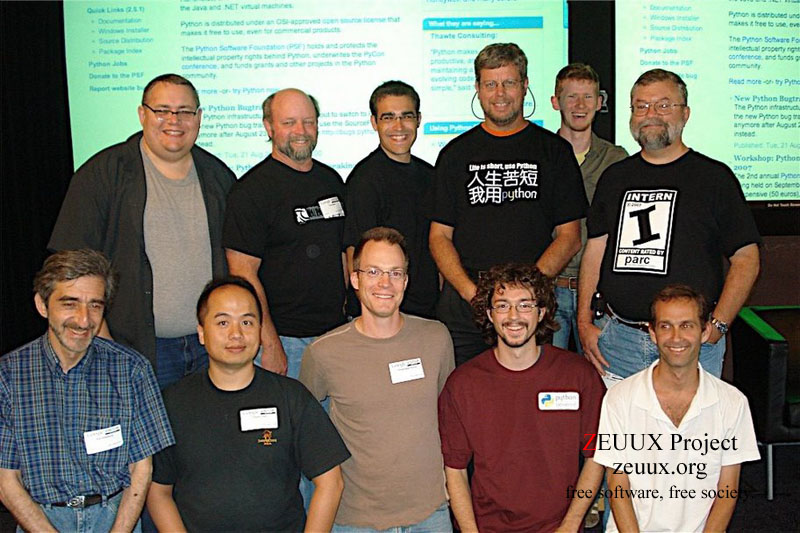
\includegraphics[height=\textheight]{guido.jpg}}
\end{frame}

\begin{frame}
  \centerline{\huge{Life is short}}
  \vspace{1cm}
  \centerline{\huge{You need Python!}}
  \vspace{1cm}
  \centerline{Bruce Eckel}
  \centerline{Author of \textit{Thinking in Java} and \textit{Thinking in C++}}
  \vspace{1.5cm}
  \centerline{\huge{人生苦短,我用Python}}
\end{frame}

\subsection{History}

\begin{frame}
  \frametitle{Brief History}
  \begin{itemize}
    \item December 1989, Guido wants a better ABC programming language
    \item October, 2000, Python 2.0 was released
    \item December, 2008, Python 3.0, a backwards-incompatible release, was
    released.
  \end{itemize}
\end{frame}

\begin{frame}
  \frametitle{Differences between Python 2 and 3}
  \begin{itemize}
    \item print is a function
    \item Views and iterators instead of lists
    \item 1/2 = 0.5; 1//2 = 0
    \item All text is unicode
    \item \ldots \ldots
  \end{itemize}
  Reference: https://docs.python.org/3/whatsnew/3.0.html
\end{frame}

\begin{frame}{Reference}
\begin{block}{Tutorials}
\begin{itemize}
  \item Google Python Class: https://developers.google.com/edu/python/?csw=1
  \item Official Documents: https://www.python.org/doc/
\end{itemize}
\end{block}

\begin{block}{Books}
  \begin{itemize}
    \item Lovely Python, 可爱的Python
    \item Think Python: How to think like a computer scientist\\
    http://www.greenteapress.com/thinkpython/thinkpython.html\\
    see thinkpython.pdf file

  \end{itemize}
\end{block}
\end{frame}

\section{Quick Get Started}
\subsection{Download and Installation}
\begin{frame}
\begin{block}{Required Softwares}
  Required softwares will be listed on GitHub before the coming
  lecture.

  https://github.com/gangchen/CUHK-I2P
\end{block}
\end{frame}

\begin{frame}
  \frametitle{Interpreters}
  \begin{block}{Various Python Interpreters}
    \begin{itemize}
      \item CPython: Official interpreter
      \item JPython: for Java Virtual Machine
      \item Ironpython: for .Net platform
      \item PyPy: just-in-time compiler
      \item Python for S60: Nokia
    \end{itemize}
  \end{block}
\end{frame}

\begin{frame}[t]{Download and installation}
  \begin{itemize}
    \item Download: www.python.org
    \item Version: Please install CPython 2.
    \item For most Linux distributions and Mac OS, Python 2.7 is preinstalled.
  \end{itemize}
\end{frame}
%--- Next Frame ---%

\begin{frame}[t]{Package Management}
  \begin{itemize}
    \item easy_install
    \item pip
  \end{itemize}
\end{frame}
%--- Next Frame ---%

\subsection{Hello Python}
\begin{frame}[fragile]
  \begin{verbatim}
    #!/usr/bin/python

    print "Hello, Python!";
  \end{verbatim}
  see HelloPython.py
\end{frame}

\begin{frame}[fragile]
  \begin{verbatim}
    python HelloPython.py
  \end{verbatim}
\end{frame}

\subsection{Python Shell}
\begin{frame}[t, fragile]{Interactive Shell}
  \begin{verbatim}
$ python
Python 2.7.6 (default, Sep  9 2014, 15:04:36)
[GCC 4.2.1 Compatible Apple LLVM 6.0 (clang-600.0.39)] on darwin
Type "help", "copyright", "credits" or "license" for more information.
>>> print "Hello Python!"
Hello Python!
>>>
  \end{verbatim}
\end{frame}
%--- Next Frame ---%




\section{Syntax}

\begin{frame}[t, fragile]{Types and Variables}
  \begin{verbatim}
    print(type(2))
    print(type(1.3))
    print(type("Hello"))

    print(type(type(1.3)))

    message = "Hello"
  \end{verbatim}
\end{frame}
%--- Next Frame ---%

\begin{frame}[t, fragile]{Operators}
\begin{verbatim}
  1.3 - 0.6 == 0.7?
  import math
  math.sqrt(2)
  math.sin(2)
\end{verbatim}
\end{frame}
%--- Next Frame ---%

\begin{frame}[t, fragile]{Package}
  \begin{verbatim}
    sin(2)
    from math import sin
    sin(2)
  \end{verbatim}
\end{frame}
%--- Next Frame ---%

\begin{frame}[t]{Conditional and loop}
  \begin{itemize}
    \item if-else
    \item for
  \end{itemize}
\end{frame}
%--- Next Frame ---%

\begin{frame}[t]{Next}
  \begin{itemize}
    \item Iteration
    \item String
    \item Lists
    \item Dict
    \item Tuples
    \item Files
    \item Object Oriented Programming
    \item \textit{Think Python} is highly recommended.
  \end{itemize}
\end{frame}
%--- Next Frame ---%

\section{iPython}
\begin{frame}[t]
  IPython provides a rich architecture for interactive computing with:
\begin{itemize}
\item Powerful interactive shells (terminal and Qt-based).
\item A browser-based notebook with support for code, text, mathematical expressions, inline plots and other rich media.
\item Support for interactive data visualization and use of GUI toolkits.
\item Flexible, embeddable interpreters to load into your own projects.
\item Easy to use, high performance tools for parallel computing.
\end{itemize}
\end{frame}
%--- Next Frame ---%

\begin{frame}[t]{matplotlib}
  \begin{block}{matplotlib}
    \begin{itemize}
      \item matplotlib is a library for making 2D plots of arrays in Python.
      \item matplotlib is designed with the philosophy that you should be able
      to create simple plots with just a few commands, or just one!
      \item Plots should look great - publication quality. One important
      requirement for me is that the text looks good (antialiased, etc.)
      \item Postscript output for inclusion with TeX documents
      \item Embeddable in a graphical user interface for application development
      \item Code should be easy enough that I can understand it and extend it
      \item Making plots should be easy
    \end{itemize}
  \end{block}
\end{frame}
%--- Next Frame ---%

\begin{frame}[t]{ipython + matplotlib}
  \centerline{\huge{ipython + matplotlib}}
  \vspace{1.5cm}
  \centerline{\huge{Python based Interactive data analysis and visualization}}
  Example: see animate_decay.py
\end{frame}
%--- Next Frame ---%


\begin{frame}[t]{Tutorial}
  \url{http://www.labri.fr/perso/nrougier/teaching/matplotlib/}
\end{frame}
%--- Next Frame ---%

\begin{frame}[t]{Next}
  \begin{itemize}
    \item scipy: a Python-based ecosystem of open-source software for scientific
    computing
    \item Biopython and other python-based bioinformatics projects
    \item Bioinformatics in the cloud: Python SDK of SBGenomics and DNAnexus
  \end{itemize}
\end{frame}
%--- Next Frame ---%

\end{document}
